\documentclass[a4paper,12pt]{article} %style de document
\usepackage[utf8]{inputenc} %encodage des caractères
\usepackage[french]{babel} %paquet de langue français
\usepackage[T1]{fontenc} %encodage de la police
\usepackage[top=2cm,bottom=2cm,left=2cm,right=2cm]{geometry} %marges
\usepackage{graphicx} %affichage des images
\usepackage{amssymb}
\usepackage{url}
\usepackage{verbatim}
\usepackage{amsmath}
\usepackage{color}
\usepackage{tikz}
\usepackage{hyperref}
\hypersetup{
	hidelinks,
    colorlinks,
    citecolor=black,
    filecolor=black,
    linkcolor=black,
    urlcolor=black
}

\begin{document} %début du document

%----------------------------------
%page de garde
%----------------------------------

\begin{titlepage}

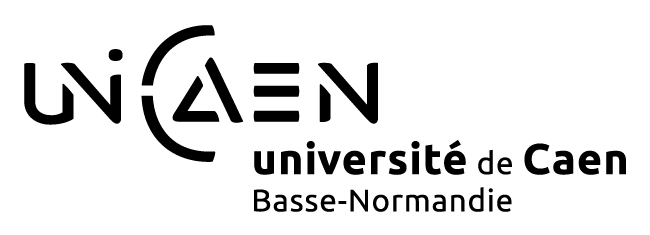
\includegraphics[scale=0.3]{images/unicaen.png}

\vspace{7cm}

\begin{center}

\begin{Huge}
Méthodes de conception\\
Rapport de Projet\\
\end{Huge}
\vspace{2cm}
\begin{large}
Beauchamp Aymeric 21301016\\
Demé Quentin 21507097\\
Jacqueline Martin 21507982\\
Zaizafoun Sami 21600538\\
\vspace{1cm}
L3 Informatique  Groupe A2
\end{large}

\end{center}
\end{titlepage}


%------------------------------
%sommaire
%------------------------------

\newpage

\tableofcontents

\newpage

%------------------------------
%contenu
%------------------------------

\section*{Présentation du projet}

L'application à développer est un jeu de stratégie au tour par tour. Chaque joueur peut se déplacer sur une grille de jeu et utiliser des armes pour vaincre ses adversaires, le but étant d'être le dernier joueur vivant.\\
Nous avons pris quelques libertés par rapport au sujet de base : chaque joueur dispose ainsi de points de vie et de points d'action, au lieu d'une simple quantité d'énergie.
Les joueurs perdent lorsqu'ils n'ont plus de points de vie, et utilisent les points d'action pendant leur tour pour effectuer leurs actions (se déplacer, tirer, utiliser le bouclier...). Les points d'action sont restitués au début du tour d'un joueur.\\
Pendant un tour, les joueurs peuvent agir autant qu'ils le veulent, tant qu'ils ont assez de points d'action pour le faire. Le tour d'un joueur se termine quand il n'a plus de points d'actions ou quand il décide de passer sans dépenser ce qui lui reste.

\section{Organisation du code}

L'application est séparée en deux packages : le package modele qui contient tout ce qui est nécessaire au fonctionnement du jeu, et le package graphics qui permet l'utilisation du jeu en interface graphique.

\begin{figure}[!h]
\centering
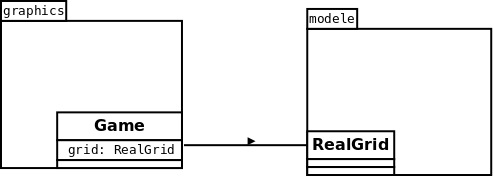
\includegraphics[scale=0.5]{images/packages.png}
\caption{Diagramme de packages}
\end{figure}

\newpage

\section{Fonctionnement du modèle}

\begin{figure}[!h]
\centering
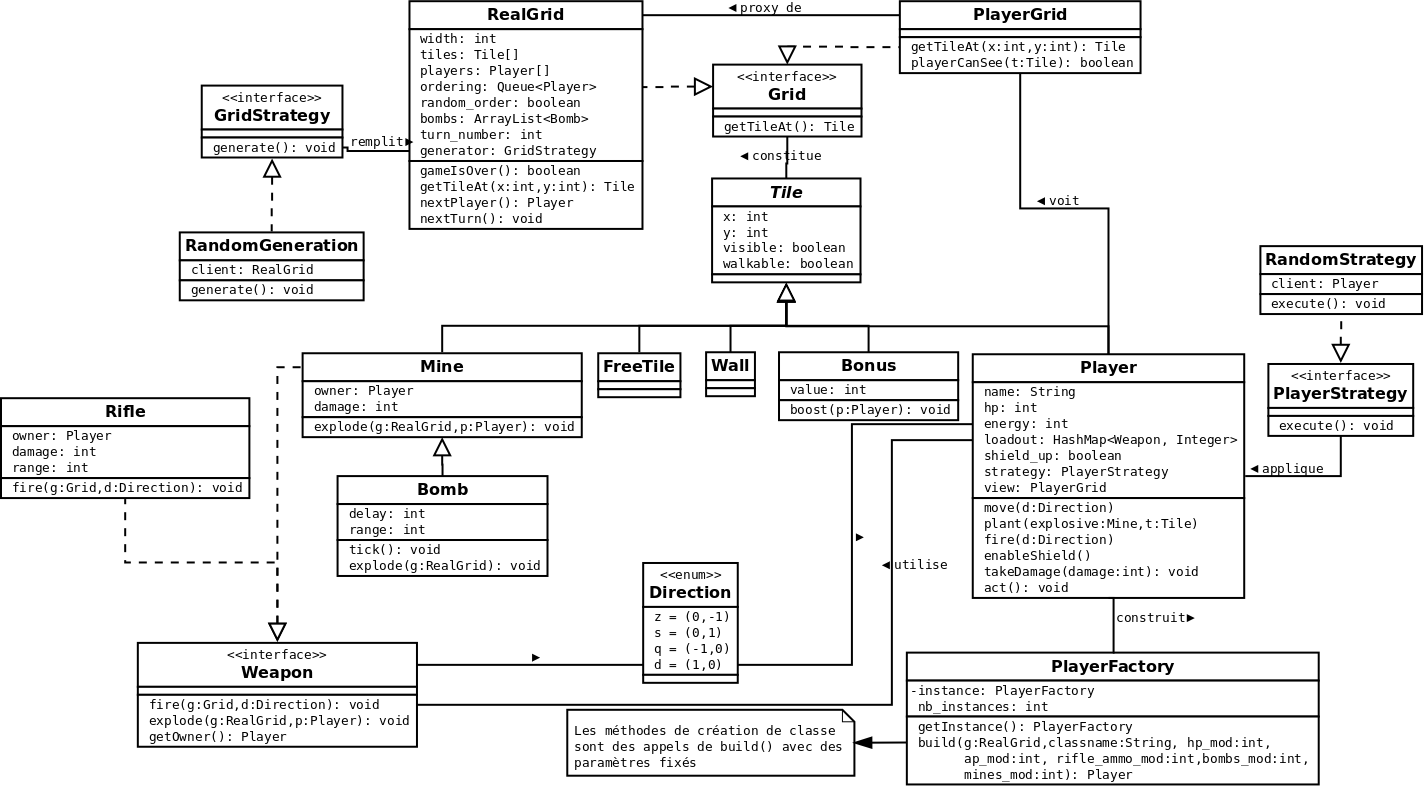
\includegraphics[scale=0.33]{images/modele.png}
\caption{Diagramme de classe du package modele}
\end{figure}

Le package modele permet de jouer au jeu en console, avec plusieurs options d'exécution.
\begin{itemize}
\item S'il est lancé sans option, on lance une partie avec 4 joueurs IA sur une grille en 10x10.
\item Avec l'option \textbf{-p0}, l'application donne accès à un menu permettant de choisir les dimensions de la grille, le nombre de joueurs et le choix de la présence d'IA ou non.
\item Avec l'option \textbf{-p1}, on a en plus la possibilité de choisir la classe de chaque joueur.
\end{itemize}


\begin{figure}[!h]
\centering
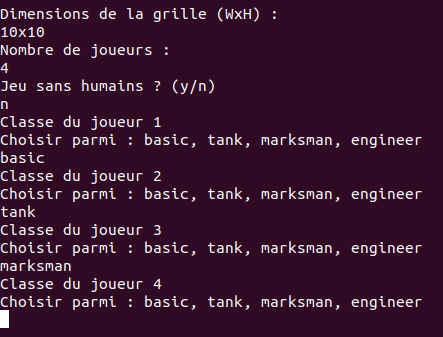
\includegraphics[scale=0.5]{images/menu.png}
\caption{Menu avancé}
\end{figure}

Le jeu est représenté par une liste de cases de différents types. Seul un type de case, les joueurs, peut modifier l'état du jeu, notamment en utilisant des armes.\\
Toutes les armes implémentent l'interface Weapon, qui contient les méthodes explode() et fire() qui effectuent respectivement une explosion et un tir. Ainsi, bien que les classes présentes n'implémentent réellement qu'une seule des deux méthodes, on peut facilement ajouter des armes à feu que l'on peut faire exploser ou des explosifs capables de tirer.\\

\begin{figure}[!h]
\centering
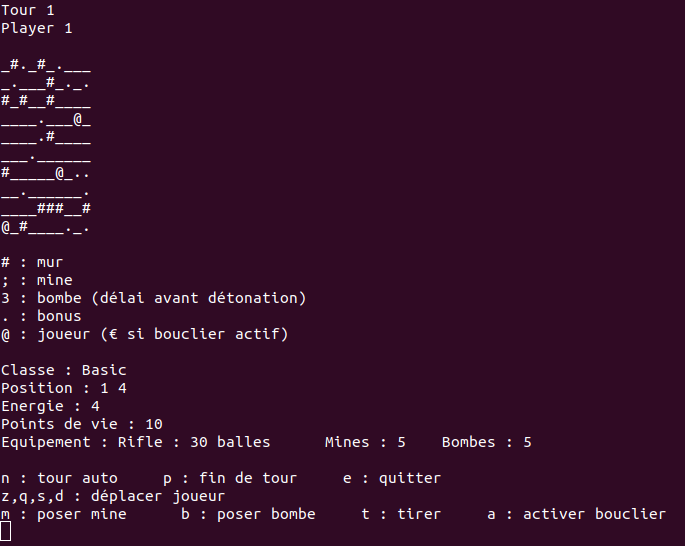
\includegraphics[scale=0.5]{images/game.png}
\caption{Interface console}
\end{figure}

\subsection{Paramétrage du jeu}

Des dégâts des armes au coût d'un déplacement, le jeu utilise de nombreuses valeurs constantes que l'on voudrait pouvoir modifier facilement dans toute l'application en une seule fois.\\
Pour ce faire, nous utilisons un fichier texte de configuration contenant des lignes au format \textit{"VARIABLE=valeur"}. La classe GameConfig lit le fichier, et stocke chaque valeur du fichier dans des variables statiques correspondantes, auxquelles on peut donc accéder depuis n'importe quelle classe.\\
Si on veut changer une valeur, il suffit de modifier le fichier de configuration et de relancer l'application sans même avoir besoin de compiler. On peut de plus proposer à l'utilisateur de modifier lui-même les valeurs s'il le souhaite, puisqu'aucune modification du code n'est nécessaire.

\subsection{Pattern factory}

L'instanciation des différents joueurs se fait via la classe PlayerFactory, qui contient une méthode \textit{build()} qui renvoie une instance de Player paramétrée par de nombreux arguments.\\
On peut ainsi facilement créer des archétypes de joueurs en définissant des méthodes appelant \textit{build()} avec des paramètres définis, par exemple un joueur résistant avec un bonus de points de vie, mais moins de munitions et d'explosifs.\\
Actuellement, les archétypes sont identifiée par une chaîne de caractère en attribut de Player, mais on pourrait également rendre la classe Player abstraite et utiliser la factory pour instancier des classes filles représentant ces archétypes.\\

\begin{figure}[!h]
\centering
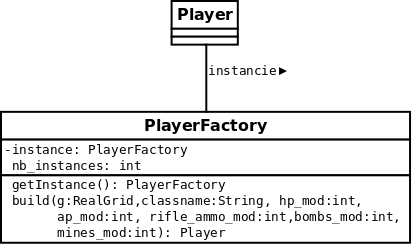
\includegraphics[scale=0.5]{images/factory.png}
\caption{Pattern factory pour les joueurs}
\end{figure}

\subsection{Pattern proxy}

Pour simplifier la mise à jour des données lorsque les joueurs agissent, il est préférable de n'avoir qu'une seule grille qui stocke toutes les informations. Cependant, on veut aussi que chaque joueur n'ait qu'une vision partielle de la grille de jeu, ne voyant que les explosifs qu'il a lui-même posés.\\
Le pattern proxy permet de réaliser ces deux impératifs en même temps. Dans notre application, nous utilisons une classe PlayerGrid qui est liée à la RealGrid unique de la partie, et à un des joueurs. Chaque joueur a donc un attribut PlayerGrid.\\
La classe PlayerGrid propose des méthodes de RealGrid modifiées pour mentir au joueur. Ainsi, là où la méthode \textit{getTileAt()} de RealGrid renvoie simplement la case se trouvant aux coordonnées demandées, la même méthode de PlayerGrid vérifie d'abord si le joueur a le droit de connaître la nature exacte de la case, et renvoie une case vide si ce n'est pas le cas. La méthode \textit{toString()} fonctionne de la même façon et permet de produire des représentations de la grille adaptées à chaque joueur.

\begin{figure}[!h]
\centering
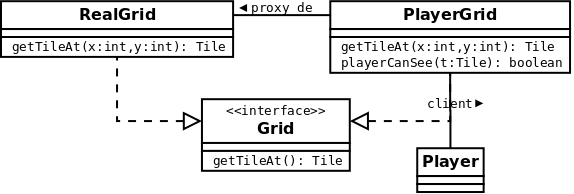
\includegraphics[scale=0.3]{images/proxy.png}
\caption{Pattern proxy pour les vues joueur}
\end{figure}

\subsection{Pattern strategy}

Nous utilisons le pattern Strategy deux fois dans l'application : pour la génération de la grille et pour le comportement de l'IA.\\
Ce pattern permet de modifier radicalement le résultat d'une méthode sans pour autant modifier le coeur du code.\\
Ainsi, la génération de grille est faite en utilisant la méthode \textit{generate()} d'une implémentation de l'interface GridStrategy. Si on veut changer la façon dont on remplit la grille, il suffit d'ajouter une nouvelle implémentation et de faire appel à un simple setter de RealGrid.

\begin{figure}[!h]
\centering
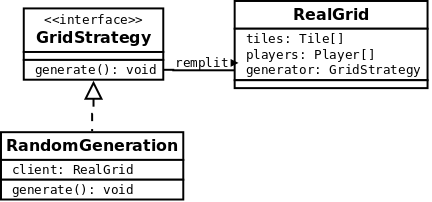
\includegraphics[scale=0.5]{images/strategy.png}
\caption{Pattern strategy pour la génération de grille}
\end{figure}


\section{L'interface graphique}
\subsection{La classe ImagesLoader}
La classe ImagesLoader est une classe s’occupant de gérer le chargement des images et de facilité leur utilisation au sein du package \textit{graphics}. Nous allons quelque peu détailler son fonctionnement.
\subsubsection{Découpage du tileset}
Les images sont découpées au sein d'une même image d'ensemble: \textit{le titeset}. Le découpage de ce tileset se fait du coin en haut à gauche, jusqu'au coin inférieur droit. Cette ordre a son importance puisque la position de l'image dans la liste correspond à l'index récupéré dans le XML moins un.
\begin{figure}[!h]
\centering
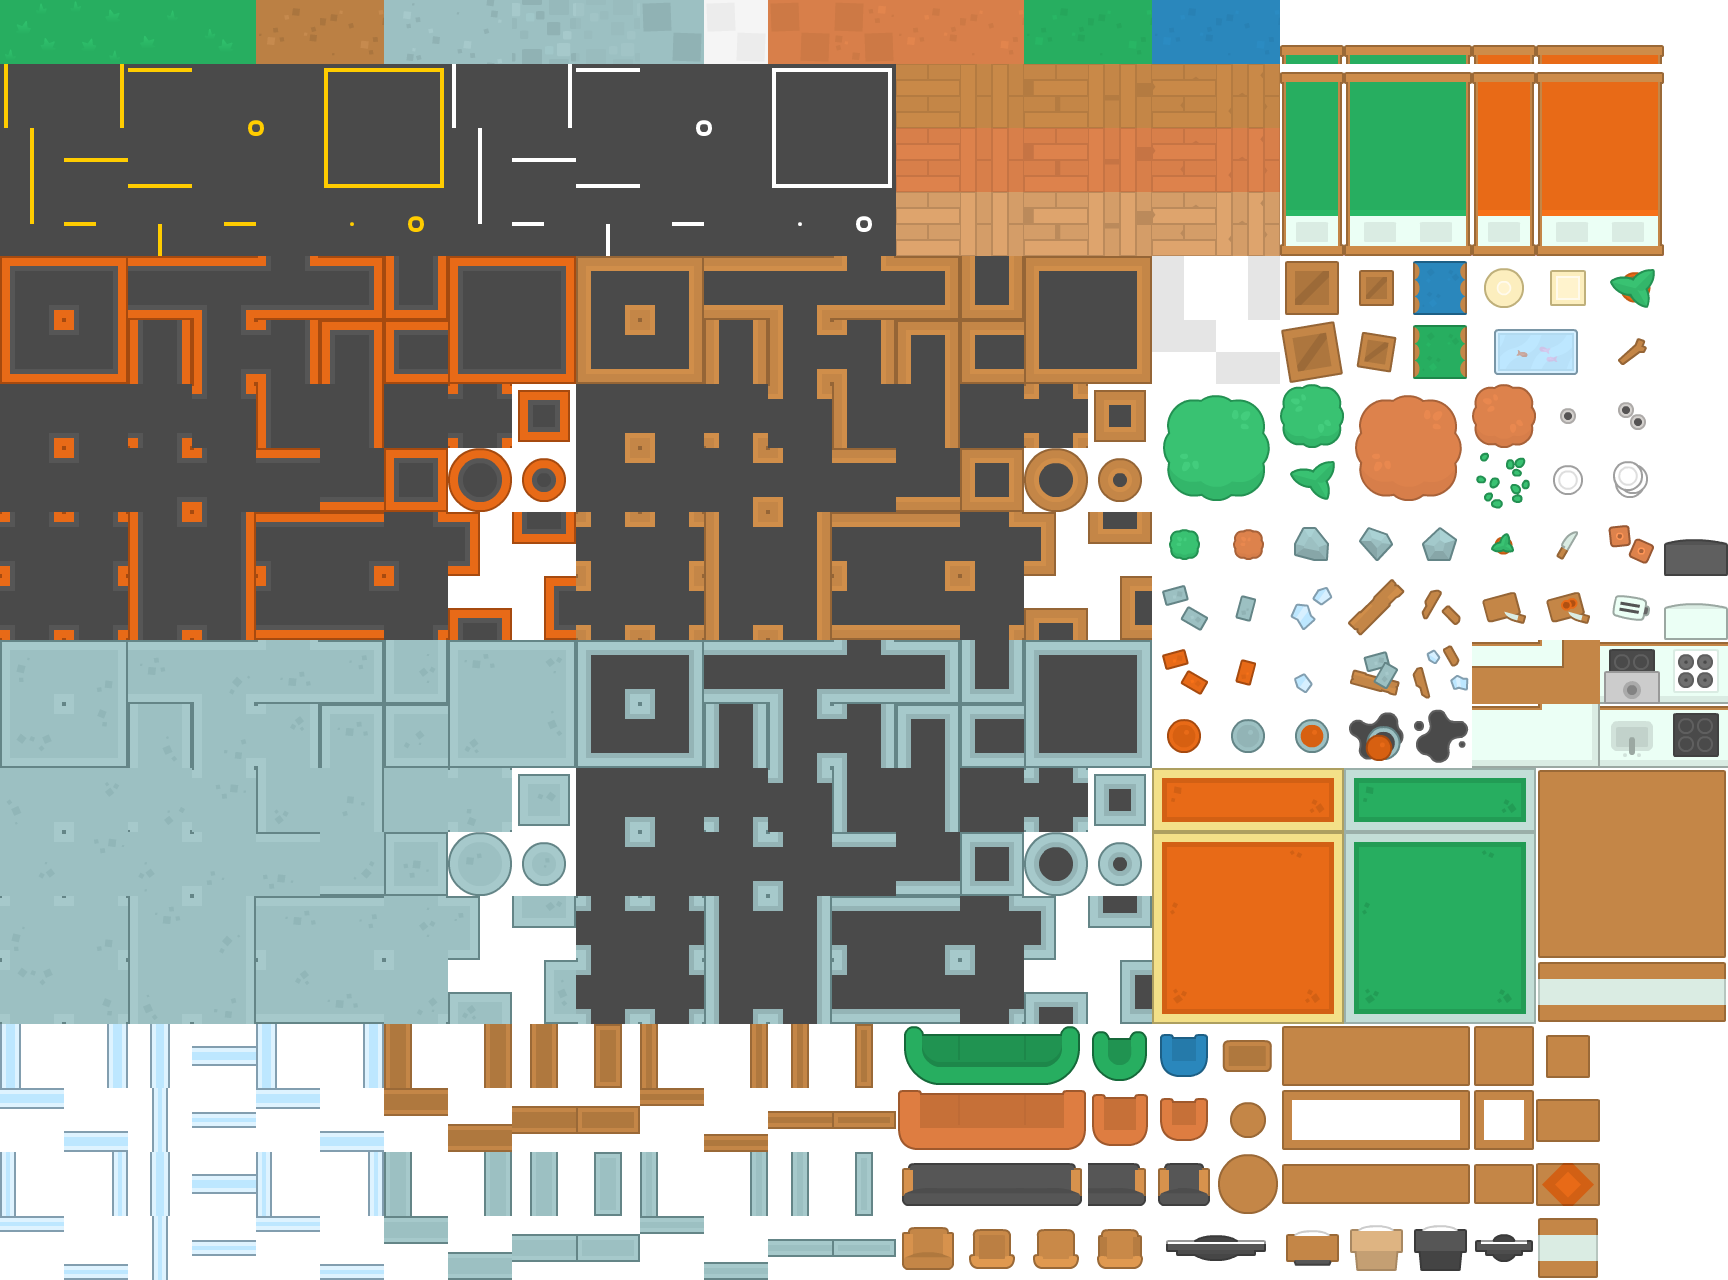
\includegraphics[scale=0.12]{images/tileset.png}
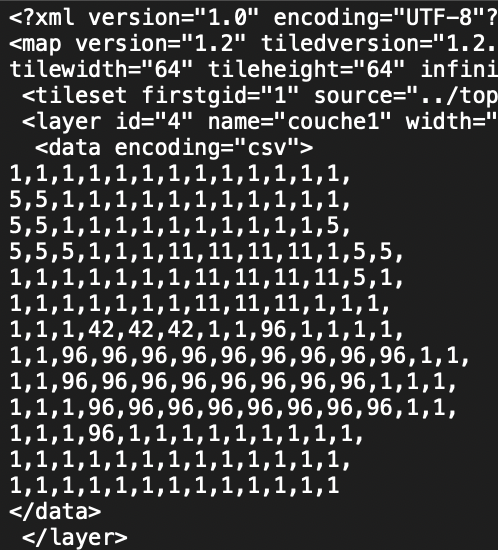
\includegraphics[scale=0.5]{images/XML.png}
\caption{Mise en parallèle du XML et du tileset}
\end{figure}
\newline
Comme on peut le voir sur la figure ci-dessus, les indices 1 correspondent à l'image 0 du tileset qui est l'image en haut à gauche de ce dernier.
\subsubsection{Utilisation}
Cette classe a pour but de charger les images nécessaires à l’affichage du jeu. Ces ressources sont créées comme étant \textit{static} pour être accessible de n’importe où sans passer par des getters. Le chargement des images nécessite tout de même un appel en début de programme de la méthode loadImages().
Ce fichier regroupe les images :
\begin{itemize}
\item Des entités d’environnement du jeu (ArrayList)
\item Des personnages (HashMap<Integer, ArrayList>)
\item Du bouclier
\item Des mines, et des bombes
\item Des bonus
\end{itemize}
Ces images sont utilisées pour créer les objets de classe \textit{Tile}. En effet, un \textit{Tile} est créée avec ses coordonnées \textit{x} et \textit{y} et une image étant sa représentation graphique.
\subsection{La classe View}
La classe view est la classe permettant l’affichage du model en vue graphique. Le code possède également une classe ViewConsole qui réalise un affichage console en permettant de jouer. 

\begin{figure}[!h]
\centering
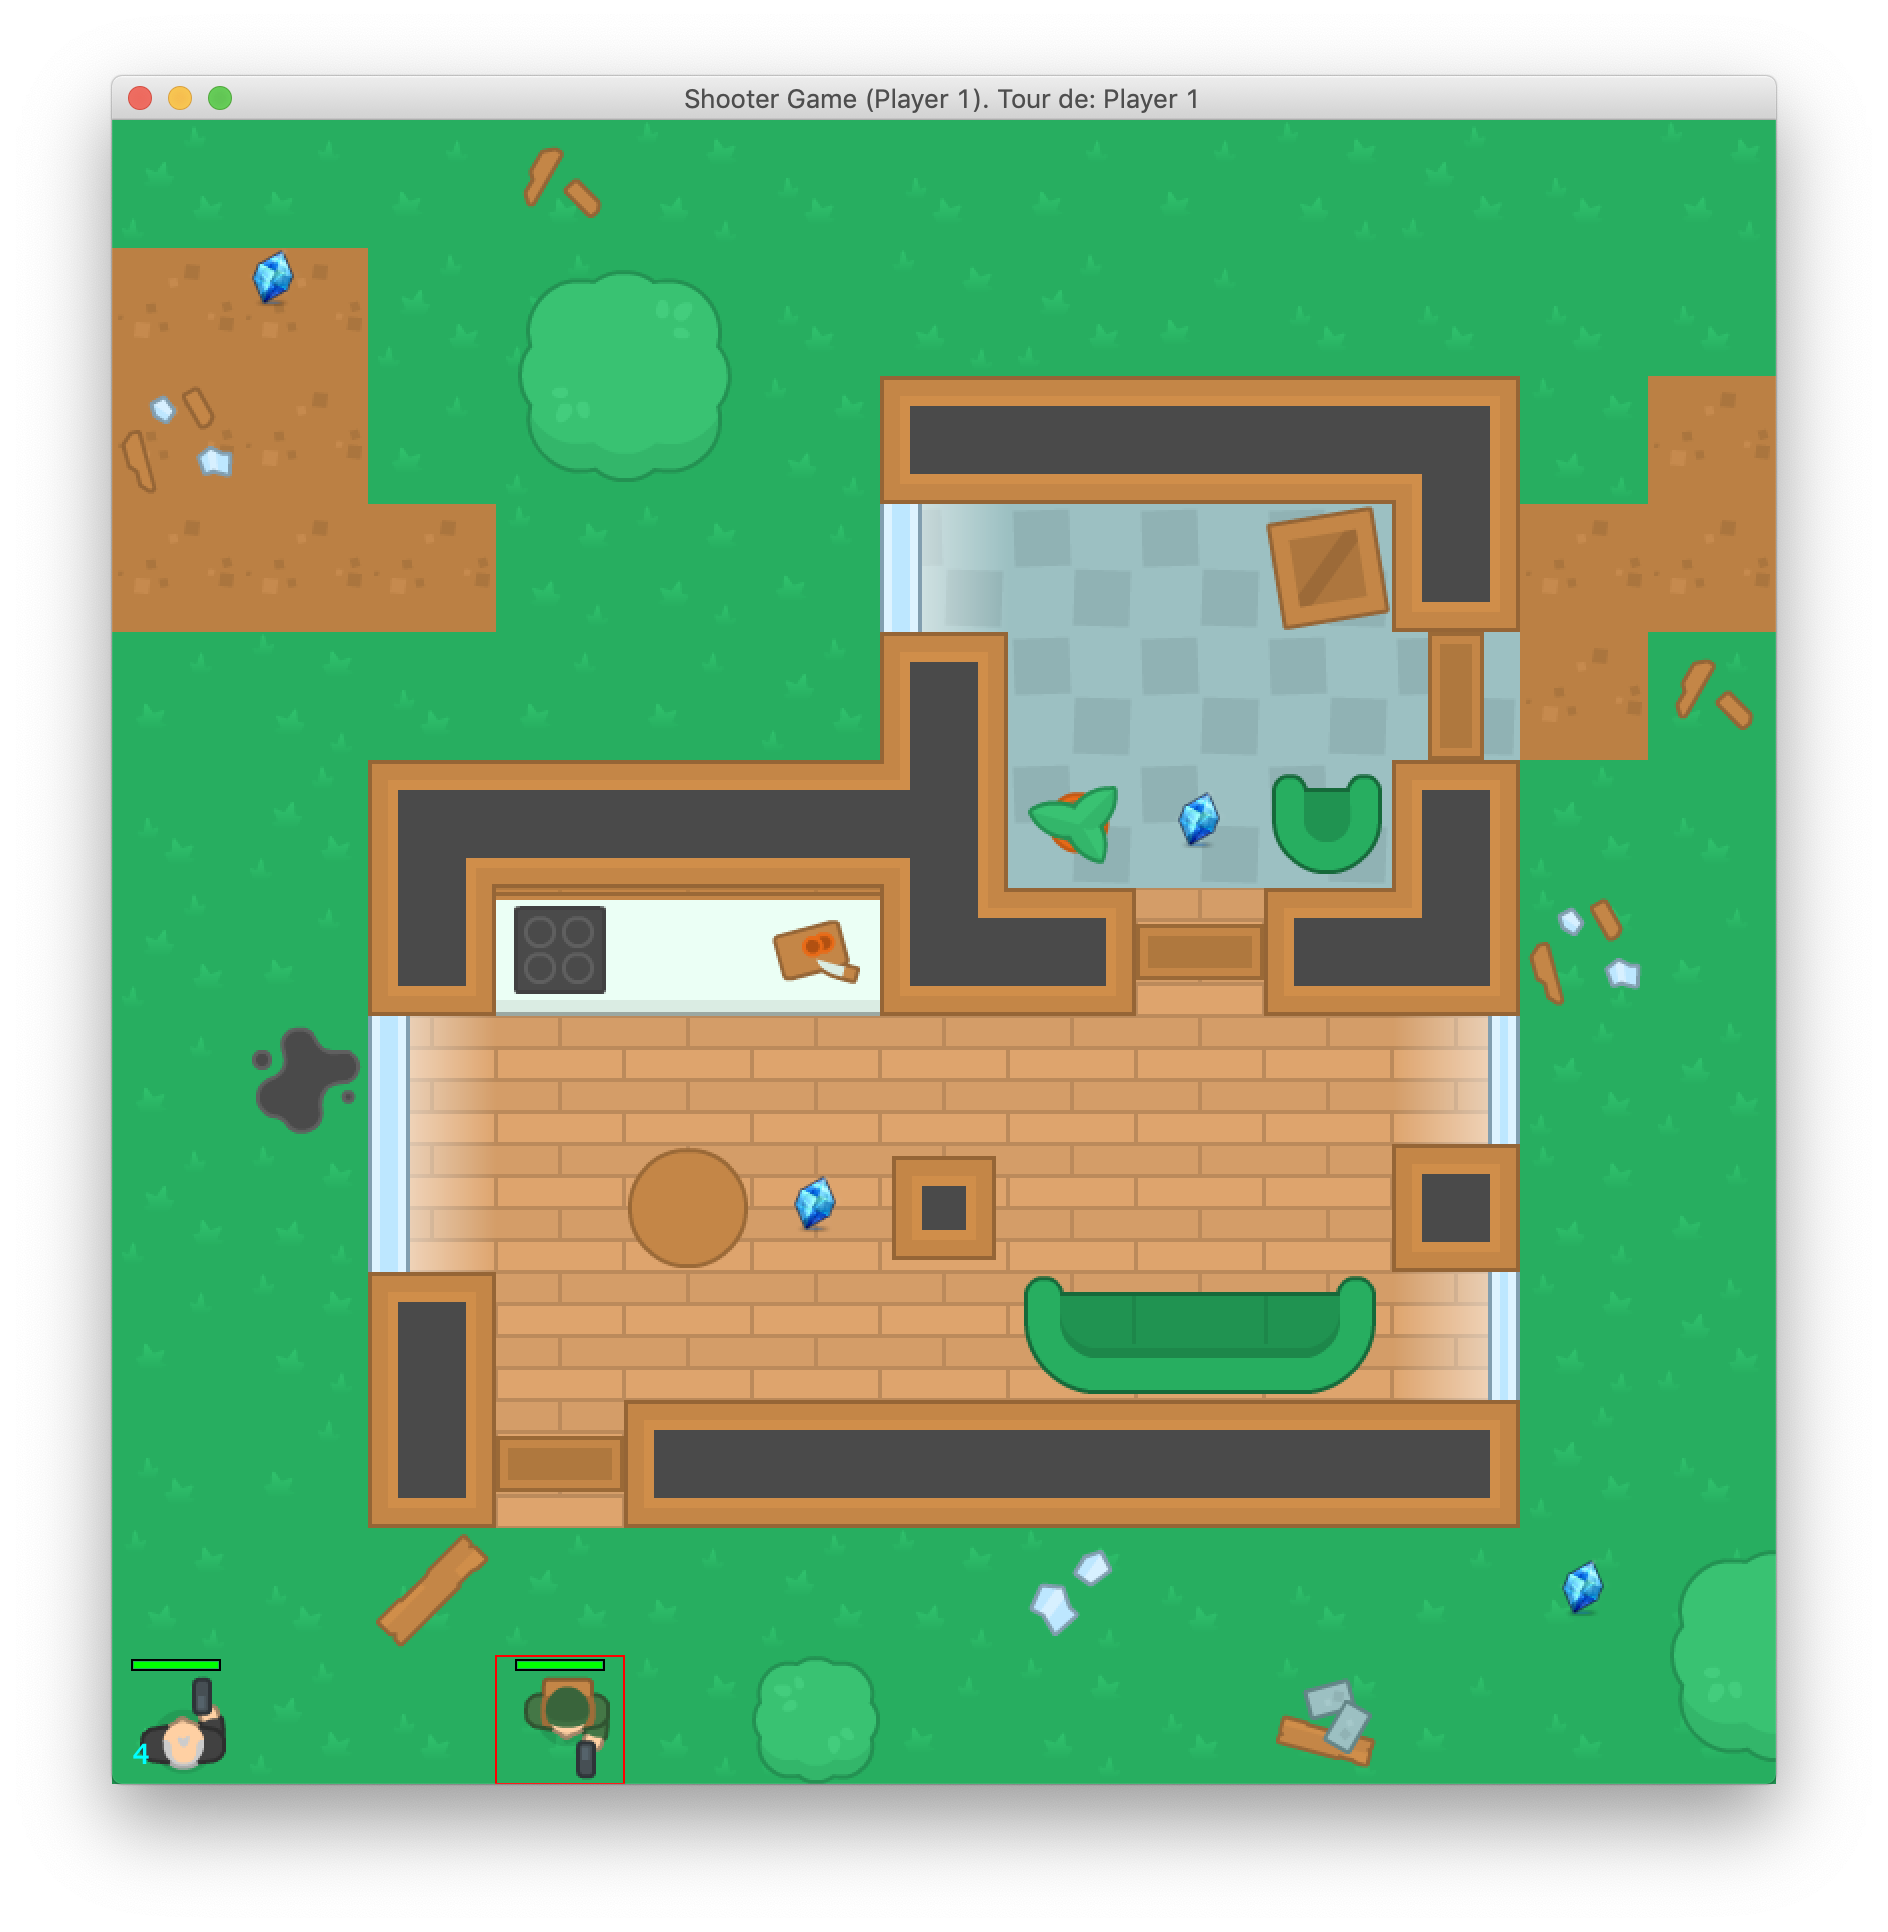
\includegraphics[scale=0.2]{images/interface.png}
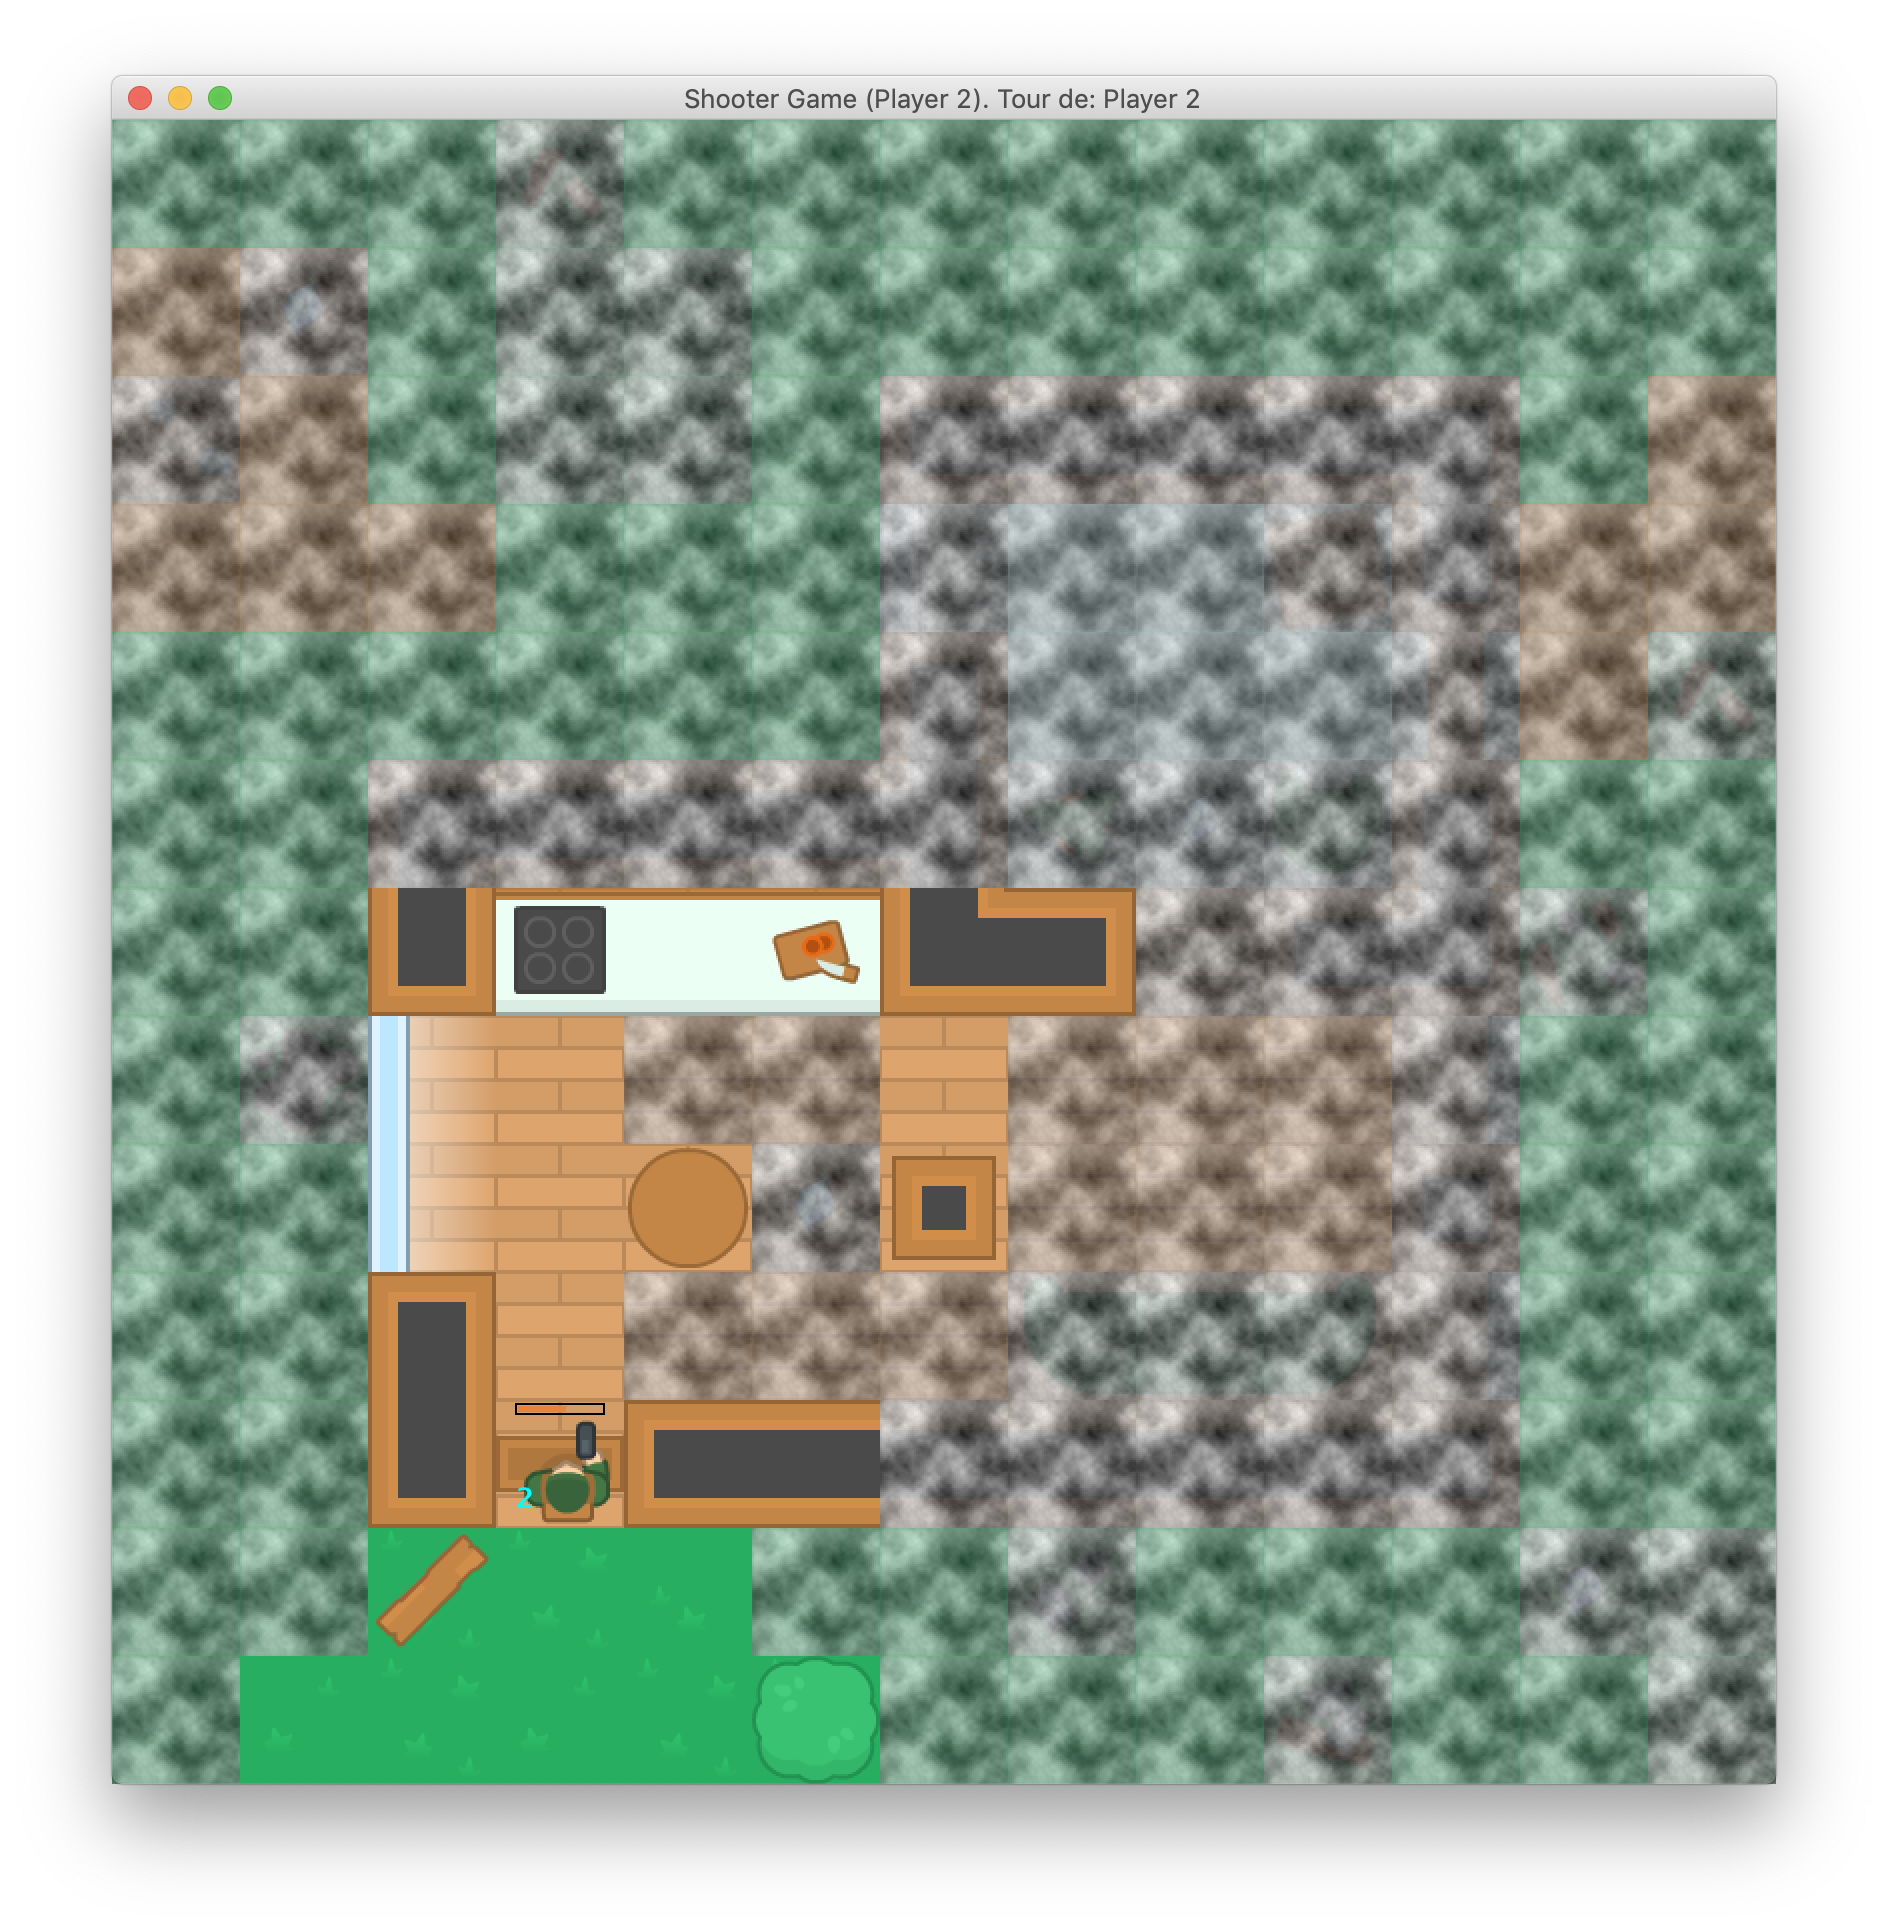
\includegraphics[scale=0.2]{images/interfaceBrume.png}
\caption{L'interface avec et sans brouillard}
\end{figure}
\subsubsection{Constructeur et principe de fonctionnement}
Lorsque la vue est créée, on renseigne pour le constructeur :
\begin{itemize}
\item Le model à écouter
\item Le joueur propriétaire de la vue
\item La liste des entités
\item la JFrame contenant la vue: l'observer
\end{itemize}
\subsubsection{Fonctionnement, affichage et actualisation.}
Lors de l’affichage, la vue parcourt la liste d'entités dans un ordre défini. Cet ordre représente notamment les couches (layers) contenues dans le fichier XML permettant de charger le niveau. L'ordre de cette liste est très important puisque l'on vient superposer les images les unes aux autres pour ajouter du détail, comme par exemple les fauteuils, tables etc.\\
Lorsque le model change, l'appel de la méthode \textit{stateChange()} provoque une actualisation de toutes les vues écoutant le model.
\subsubsection{Un élément optionnel : l’animation de tir}
Lorsqu'un joueur tir, une animation se déclenche permettant de visualiser le parcours de sa balle. Cette animation est réalisée par le biais d'un Thread actualisant deux valeurs x et y tant que la portée maximale n'a pas été atteinte. A chaque actualisation, on prévient la vue pour qu'elle puisse se repeindre. La classe permettant cette animation est la classe \textit{ThreadPlay}. 
\subsection{La classe GUI}
La classe GUI est la classe permettant de créer une fenêtre accueillant la vue d'un joueur.
\subsubsection{Constructeur et principe du fonctionnement}
Lors de sa création cette classe reçoit en argument:
\begin{itemize}
\item Le modèle
\item Le joueur à qui la vue devra appartenir
\end{itemize}
La vue est ensuite créée au sein du constructeur.
\subsubsection{La jouabilité}
L'application est jouable au clique et au clavier. En effet pour chaque action le joueur doit d'abord cliquer sur son personnage pour faire afficher un menu déroulant de ses actions possibles. Toutefois, si le joueur souhaite effectuer plusieurs déplacements à la suite.
\subsubsection{Entrées claviers}
Pour lire les entrées claviers, on doit dans un premier temps invoquer la méthode \textit{setFocusable(true)} puis la méthode \textit{requestFocus()}. Puis ajouter un keyListener a la fenêtre. 
\subsubsection{Entrées souris}
La majorité des actions se font grâce aux cliques. Pour cela, on ajoute un \textit{mouseListener} à la fenêtre. Ensuite on agit en conséquence lorsque l'on reçoit un clique.
\subsection{Player}
\subsubsection{line of sight : visiblesTiles}
Cette fonction est originellement utilisée comme test pour la ligne de vue des joueurs. Son principe est la base du suivant. Il test uniquement les directions cardinales dans quatre boucles \textit{while} qui s'arrêtent si elles rencontrent un mur ou si elles sont arrivées à la limite de taille de vue (\textit{visionSize}).
\subsubsection{line of sight : testView}
Dans \textit{testView()} nous testons si la case indiqué est visible par le joueur, pour cela, nous considérons une grille temporaire composée de 0, nous allons ensuite calculer la distance en case qui sépare nos deux points, puis les vecteurs, nous décomposeront ce vecteur en plusieurs que nous appliquerons 1 par 1, a chaque application, nous approchons du point testé, et a  chaque avancé, nous ajoutons +1 a la grille, dans la case équivalent à la où nous nous situons, cela permet de connaître les cases parcourues (voir schéma) si dans la boucle des cases parcourues, nous observons une Tile qui a sont attribut \textit{isWalkable} à \textit{faux}, alors la fonction \textit{testView} est arretée. Dans le cas contraire, si elle fini la boucle, alors nous sommes bien arrivé à la case testée, nous pouvons donc l'ajouter dans la liste des cases visibles.
\subsubsection{line of sight : visibleTiles}
La fonction \textit{visiblesTiles()} quand à elle fait deux choses, en premier lieu elle appelle \textit{testView} pour chaque case, ensuite, elle teste tout les murs afin de savoir si une case adjacente est visible, si c'est le cas alors le mur sélectionné le deviens aussi, cela permet au joueur de comprendre ce qui  bloque son champs de vision.
\subsubsection{line of sight : notes}
Dans la gestion de la ligne de vue, nous utilisons finalement les deux fonctions renvoyant les Tuiles visibles, \textit{visibleTiles} et \textit{visiblesTiles} pour éviter toute possibilité de bug dans les zones proches dûes à la gestion des lignes, celle-ci pouvant sembler anormale pour l'humain, mais pour autant mathématiquement exacte.
\begin{figure}[!h]
\centering
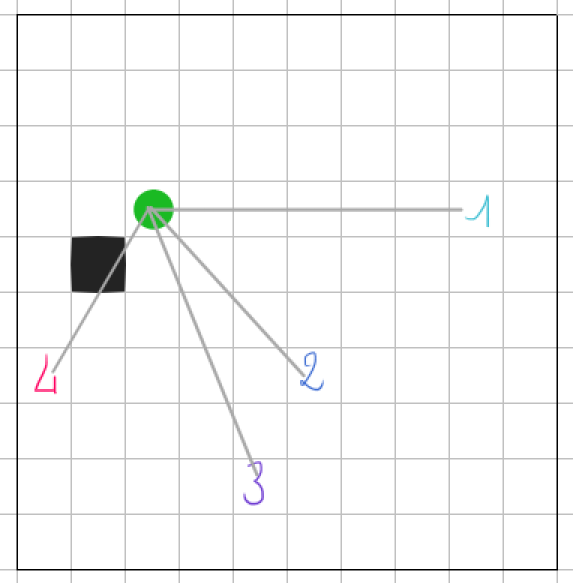
\includegraphics[scale=0.2]{images/ex1.png}
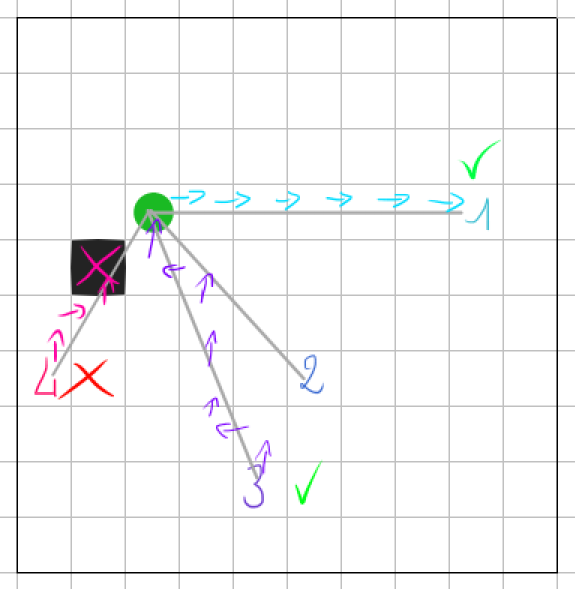
\includegraphics[scale=0.2]{images/ex2.png}
\caption{exemple de fonctionnement de plusieurs \textit{testView}}

\end{figure}

\end{document}